% vkGSplat: A Compute-First Vulkan Path for Robotics Synthetic Data
% Position / vision paper draft (v0.1)
% Target venue: HotOS-style position track, HPG, MLSys, or arXiv preprint.

\documentclass[10pt,journal]{IEEEtran}

\usepackage{graphicx}
\usepackage{amsmath,amssymb}
\usepackage{array}
\usepackage{booktabs}
\usepackage{hyperref}
\usepackage{cite}
\usepackage{xcolor}
\usepackage{url}
\usepackage{tikz}
\usepackage{pgfplots}
\usetikzlibrary{positioning,arrows.meta,shapes.geometric,backgrounds,fit,calc}
\usepgfplotslibrary{fillbetween}
\pgfplotsset{compat=1.18}

\newcommand{\todo}[1]{\textcolor{red}{[TODO: #1]}}
\newcommand{\note}[1]{\textcolor{blue}{[NOTE: #1]}}
\definecolor{plotblue}{RGB}{30,144,255}
\definecolor{plotcyan}{RGB}{0,180,190}
\definecolor{plotgreen}{RGB}{0,160,90}
\definecolor{plotyellow}{RGB}{235,180,35}
\definecolor{plotred}{RGB}{210,70,70}

\title{vkGSplat: A Compute-First Vulkan Path for\\Physical AI World Simulation and Synthetic Data Generation}

\author{%
    Chien-Ping Lu\\[0.35em]
    \normalsize May 4, 2026%
}

\begin{document}
\maketitle

\begin{abstract}
Modern robotics increasingly depends on synthetic data generated inside
photorealistic digital twins. The dominant pipelines --- NVIDIA Isaac~Sim
\slash Omniverse, Cosmos, BlenderProc, Kubric --- bind the rendering layer to
graphics-optimized silicon: GPUs with rasterizers, ROPs, and ray-tracing
cores. We argue that this binding is incidental rather than fundamental.
The trend is already visible inside graphics itself: the GPU has evolved
from a fixed-function graphics processor into a programmable graphics,
scientific-computing, and AI platform~\cite{dally2021gpu}, while DLSS and
its peers have shifted the center of gravity of real-time rendering from
fixed-function graphics units to \emph{tensor compute}. In this newer
model, the rasterizer and RT cores increasingly act as an
\emph{acquisition} stage that produces low-resolution, temporally and
spatially sparse measurements; neural and classical reconstruction then
upscales, denoises, anti-aliases, and
interpolates~\cite{nvidia-dlss,liu2020nsrr,nvidia-dlss3,schied2017svgf,bitterli2020restir}.
Synthetic data generation (SDG) is a \emph{throughput-bound,
latency-tolerant} workload, and its rendering quality requirements --- while
non-trivial --- are met by published compute-only techniques (software
rasterization, GPU ray traversal, 3D Gaussian splatting) that do not require
fixed-function graphics hardware. We propose \textbf{vkGSplat}: a Vulkan
implementation in which the API surface is preserved as a portable contract,
but the backend is a software renderer expressed in CUDA-class compute. The
near-term motivation is access: data-center AI accelerators (H100, B200, AI
chips such as TPU and Trainium) are over an order of magnitude more available,
in aggregate FLOPS and procurement velocity, than RTX-class workstation
silicon. The longer-term motivation is portability: decoupling the API from
the silicon turns digital-twin pipelines into a software problem with a clean
backend interface. We present the system design, situate it relative to
existing software-Vulkan implementations (SwiftShader, Mesa Lavapipe), justify
3D Gaussian Splatting as the v1 renderer, and lay out an evaluation plan for
throughput, energy, and downstream sim-to-real task accuracy. As a
design target, we aim for \textbf{$\geq 100$ images\slash s\slash H100} at
$1024{\times}1024$ from a captured 3DGS scene, \textbf{$\leq 0.5$ J\slash
image} on H100-class hardware, and \textbf{within $2{\times}$ of an
RTX-class graphics-hardware baseline (L40) on dollars per image} ---
benchmarked against Isaac~Sim and BlenderProc on identical scene
geometry. These targets are extrapolations from published 3DGS
throughput on RTX-class hardware~\cite{kerbl20233dgs} and from the
software-rasterization literature~\cite{laine2011software}; achieving
them is the v1 falsifiable claim.
\end{abstract}

\begin{IEEEkeywords}
Synthetic data generation, Vulkan, software rendering, 3D Gaussian splatting,
digital twins, robotics, AI accelerators.
\end{IEEEkeywords}

% =====================================================================
\section{Introduction}
% =====================================================================

Two trends are colliding. First, robotics has become a data-hungry
discipline: end-to-end visuomotor policies, foundation models for
manipulation, and autonomy stacks all require enormous quantities of
labeled visual data, and an increasing fraction of that data is
\emph{synthetic} --- rendered inside high-fidelity simulators
\cite{tobin2017domain,greff2022kubric,denninger2019blenderproc,deitke2022procthor}.
Second, the silicon supply chain has bifurcated: AI accelerators
(NVIDIA~H100\slash B200, Google~TPU, AWS Trainium, and a long tail of
emerging chips) are scaling FLOPS and memory bandwidth at a pace that
outstrips the workstation-class GPUs traditionally used for graphics, and
they dominate procurement budgets at every hyperscaler.

The collision is awkward. Today's leading SDG stacks --- NVIDIA
Omniverse\slash Isaac~Sim\slash Replicator and Cosmos
\cite{nvidia2024cosmos}, Unreal-based platforms, Blender-based pipelines
\cite{denninger2019blenderproc,greff2022kubric} --- are built on graphics
APIs (Vulkan, D3D12, Metal, OpenGL) whose performant implementations
require dedicated graphics silicon: rasterizer pipelines, ROPs, RT cores.
The data-center accelerators that companies actually have are largely
graphics-blind: an H100 has no RT cores, and TPUs and Trainium have no
graphics pipeline at all. Generating training data on the chips one
already owns therefore requires either (a) provisioning a separate fleet
of graphics GPUs or (b) abandoning the graphics-API ecosystem in favor of
custom rendering harnesses, which fragments the tooling.

This paper takes the position that this fragmentation is unnecessary.
Vulkan is a clean, modern, vendor-neutral API. There is no fundamental
obstacle to implementing it as a \emph{software renderer expressed in
compute kernels}, lowering rasterization, ray tracing, and shadow mapping
to general-purpose accelerator compute. Software Vulkan implementations
already exist (SwiftShader~\cite{swiftshader}, Mesa
Lavapipe\slash llvmpipe~\cite{mesa-lavapipe}), but they target CPUs for
correctness and conformance, not GPUs for throughput; they do not exploit
the parallelism of AI accelerators, and they have not been engineered for
SDG workloads. We propose to fill that gap.

The argument has, in fact, already been made by the
graphics-hardware industry's own roadmap. In modern real-time pipelines
exemplified by NVIDIA DLSS~\cite{nvidia-dlss,liu2020nsrr,nvidia-dlss3},
the rasterizer and RT cores no longer produce the final image: they
produce a \emph{low-resolution, temporally jittered, spatially sparse,
under-sampled path-traced seed}. The rest of the pipeline ---
super-resolution, anti-aliasing, denoising, frame
interpolation~\cite{schied2017svgf,chaitanya2017interactive,nvidia-nrd},
and importance-resampled direct illumination~\cite{bitterli2020restir} ---
runs on tensor units. Each generation of DLSS shrinks the seed and
expands the neural reconstruction. \emph{The center of gravity of the
real-time rendering pipeline has already moved off fixed-function
graphics hardware and onto tensor compute.} What we propose is the
logical next step: if the AI portion is doing the heavy lifting, replace
the fixed-function seed generator with a software-rendered seed produced
on the same tensor-rich silicon, and eliminate the dependence on
graphics-specific units altogether. For SDG, where real-time interaction
is unnecessary, this trade is straightforward.

This does not require vkGSplat to clone DLSS. DLSS is the precedent that
motivates moving reconstruction work onto compute, not a required
implementation dependency. The near-term vkGSplat stack now prioritizes
Vulkan/SPIR-V capture, low-sample ray-tracing seed frames, classical
temporal reprojection, history rejection, TAA, and denoising. 3D
Gaussian Splatting remains an optional backend and research
representation, but it is not on the default implementation path. A
learned DLSS-like temporal reconstruction model is reserved for optional
later research if these deterministic passes prove insufficient.

\textbf{Relation to the Gaussian reconstruction note.} This paper should
not carry the full 3DGS reconstruction argument. Its role is to define
the compute-first Vulkan/SDG system boundary: application capture,
software acquisition, seed buffers, backend portability, and the
hardware-allocation thesis. The companion technical note on integrated 3DGS reconstruction owns the
question of whether one persistent 3D/4D Gaussian state can unify Monte
Carlo denoising, radiance caching, temporal AA, super-resolution, and
frame interpolation. In other words, this paper treats 3DGS as a
backend and possible reconstruction representation; the companion note
works out the Gaussian-state math and CUDA experiments.

\textbf{Contributions.} This is a position paper introducing the
\textbf{vkGSplat} project. We make six claims:

\begin{enumerate}
    \item \textbf{Graphics model.} Modern graphics is no longer best
    understood as a monolithic raster pipeline. It is an acquisition
    front-end --- primary visibility, shadow or light visibility,
    secondary visibility, depth, motion, and sparse radiance --- followed
    by reconstruction. This is the architectural reason a Vulkan program
    can be lowered to compute kernels without changing its role in the
    SDG stack (Section~\ref{sec:acqrec}).

    \item \textbf{Allocation law.} The modernized Amdahl argument says
    that fixed-function specialization faces a finite collapse threshold
    when the value-scalable fraction of a workload grows. In vkGSplat,
    bounded visibility becomes acquisition, while reconstruction remains
    the scalable stage that should stay on programmable compute
    (Section~\ref{sec:amdahl-main} and Appendix~\ref{app:amdahl}).

    \item \textbf{Workload.} Robotics SDG is throughput-bound and
    latency-tolerant. A renderer that produces images in tens to hundreds
    of milliseconds is acceptable if it sustains high aggregate throughput
    and high quality. This relaxes the constraint that historically
    forced the use of fixed-function graphics hardware
    (Section~\ref{sec:workload}).

    \item \textbf{API decoupling.} The Vulkan API can be preserved as the
    application contract while the implementation is replaced by a
    compute-only software renderer. We outline the architecture of such
    an implementation (Section~\ref{sec:design}).

    \item \textbf{Ray-tracing seed path before 3DGS.}
    The active v1 implementation targets low-sample, Vulkan-ray-tracing
    shaped seed frames before returning to 3DGS. This keeps the project
    focused on taking existing Vulkan programs, preserving SPIR-V and
    camera/depth/primitive contracts, and lowering reconstruction work
    to CUDA-friendly tile kernels. The earlier tile-based 3DGS renderer
    remains available as an optional backend, but no longer gates the
    main milestones (Section~\ref{sec:v1}).

    \item \textbf{Hardware-agnostic backend.} The compute IR underlying
    the renderer can be retargeted from CUDA to SYCL, Triton, or
    AI-accelerator native APIs, broadening deployment to any chip with
    sufficient compute and memory bandwidth (Section~\ref{sec:backends}).
\end{enumerate}

\textbf{System goals.} The implementation goal is not merely to run a
toy renderer on CUDA; it is to make existing Vulkan programs and
compute backends coexist behind one stable contract. Concretely, vkGSplat
aims to:

\begin{enumerate}
    \item \textbf{Preserve Vulkan as the application boundary.}
    Applications should continue to create Vulkan pipelines, descriptor
    sets, command buffers, SPIR-V modules, acceleration structures, and
    frame resources. The compatibility burden belongs inside vkGSplat,
    not in per-application ports.

    \item \textbf{Make SPIR-V and backend kernels share one ABI.}
    Every captured shader module should lower to an explicit kernel
    interface describing entry points, descriptor sets, bindings,
    storage classes, push constants, built-ins, and opaque resources
    such as TLAS handles. CPU reference kernels, CUDA kernels, and
    portability backends must consume the same interface rather than
    maintaining parallel hand-written bindings.

    \item \textbf{Use CUDA as the production backend.} The long-term
    target remains NVIDIA data-center CUDA execution, including
    CUDA-friendly tile scheduling, software BVH traversal, temporal
    reconstruction, denoising, and eventually direct Vulkan--CUDA
    synchronization and memory interop.

    \item \textbf{Use CPU and Metal as correctness backends.} CPU
    kernels define the portable reference behavior. Metal on Apple
    Silicon is a local native-GPU check that the contracts are not
    accidentally CUDA-only before the CUDA implementation is complete.

    \item \textbf{Keep the renderer tile based.} Rasterization,
    ray-tracing seed generation, reprojection, denoising, and optional
    3DGS blending should all be organized as tile- or block-local work
    so the algorithms map naturally to CUDA thread blocks and can later
    be retargeted to SYCL, Triton, or accelerator-native compute.
\end{enumerate}

\textbf{Non-goals.} vkGSplat is not aimed at real-time gaming, VR, or
display-bound interactive workloads. We do not claim to outperform RTX
hardware on its own ground. We claim only that, for the SDG workload,
running graphics on AI compute is viable, economically attractive, and
strategically preferable.

\textbf{Prototype status.} The current implementation is deliberately
CPU-first while preserving the CUDA target. It includes a portable
Wicked Engine Vulkan capture harness, restricted SPIR-V analysis and
C/CUDA translation tests, camera-derived temporal reprojection with
depth and primitive-ID history rejection, an SVGF-style denoising
baseline, a Vulkan-ray-tracing-shaped CPU seed fixture, and a first
native Metal compute backend for Apple Silicon. The
tile-binned 3DGS reference renderer is kept behind an explicit build
flag rather than being part of the default path. On the local MoltenVK
test machine the Wicked harness loads the target scene and reports
SPIR-V shader format, but mesh shaders and Vulkan ray tracing are not
exposed; therefore the current ray-tracing work uses
Vulkan-API-shaped fixtures until a backend with the required extensions
is available. The first such fixture implements a small triangle-scene
seed tracer that emits the same color, depth, NDC-depth, and
primitive-ID buffers expected from a
\texttt{VK\_KHR\_ray\_tracing\_pipeline} capture, then feeds those
buffers through temporal reprojection and denoising. This staging keeps
correctness testable on CPUs while the data layouts and algorithms
remain tile-friendly for CUDA.

% =====================================================================
\section{Background}\label{sec:bg}
% =====================================================================

\subsection{Synthetic data generation for robotics}

The use of simulated environments to train physical agents predates deep
learning, but its modern form was crystallized by domain
randomization~\cite{tobin2017domain} and by simulation platforms such as
Habitat~\cite{savva2019habitat}, ThreeDWorld~\cite{gan2020threedworld},
ProcTHOR~\cite{deitke2022procthor}, and NVIDIA Isaac~Sim. Recent SDG
toolkits like BlenderProc~\cite{denninger2019blenderproc} and
Kubric~\cite{greff2022kubric} provide higher-level scripting for
photorealistic image and video generation with controlled randomization
of geometry, materials, and lighting. NVIDIA Cosmos~\cite{nvidia2024cosmos}
extends this trajectory by combining classical rendering with generative
priors. Across these systems, the rendering layer is the single largest
silicon dependency.

\subsection{Software Vulkan implementations}

Two production software-Vulkan implementations exist.
\textbf{SwiftShader}~\cite{swiftshader}, originally a software renderer
project at TransGaming and now maintained by Google, provides a portable,
LLVM-JIT-based Vulkan~1.3 implementation that runs on CPUs (it is shipped
in Chromium for fallback rendering). \textbf{Mesa Lavapipe}~\cite{mesa-lavapipe}
is the Vulkan front-end on top of Mesa's \texttt{llvmpipe} CPU rasterizer.
Both are correctness-first and CPU-targeted; their performance on GPUs is
either non-existent (Lavapipe is CPU-only) or limited (SwiftShader has
experimental Reactor backends but is not optimized for AI-accelerator
throughput). Neither targets the SDG workload class.

\subsection{Compute-only graphics on GPUs}

There is a long line of research in software rendering on
general-purpose GPU compute. Laine and
Karras~\cite{laine2011software} showed that a fully software rasterizer
on CUDA could approach hardware rasterizer throughput for many workloads,
particularly when rasterization was not the bottleneck.  The same
lineage survives in \textsc{nvdiffrast}~\cite{laine2020nvdiffrast}, which
packages CUDA-accelerated rasterization, interpolation, texturing, and
antialiasing as low-level differentiable rendering primitives.
For ray tracing, Aila and Laine~\cite{aila2009understanding} established
the architectural patterns that would later become OptiX~\cite{parker2010optix}
and Embree~\cite{wald2014embree}. Path tracers including
Mitsuba~3~\cite{jakob2022mitsuba3} (built on Dr.Jit~\cite{jakob2022drjit})
and Falcor~\cite{benty2020falcor} demonstrate that high-quality,
differentiable rendering can be expressed entirely in compute.
Meanwhile, 3D Gaussian Splatting~\cite{kerbl20233dgs} and its
descendants~\cite{yu2024mip,huang20242dgs,ye2024gsplat} have established a new class
of renderer that is compute-native by construction.

The intellectual point is simple: every major step of a modern graphics
pipeline has a published, competitive software-on-compute implementation.
\textbf{What does not exist is a unified Vulkan front-end that exposes
these implementations through a standard API to existing graphics
applications.} That is the gap vkGSplat targets.

% =====================================================================
\section{Modern graphics as acquisition and reconstruction}
\label{sec:acqrec}
% =====================================================================

The standard account of GPU evolution is that fixed-function graphics
hardware became programmable shaders, programmable shaders became
general-purpose compute, and GPUs became a shared substrate for
graphics, scientific computing, and AI. Dally, Keckler, and Kirk tell
this hardware story directly: the GPU began as a dedicated real-time
graphics processor, then accumulated programmability, floating-point
performance, resilience, and AI-scale throughput as new users mapped
their workloads onto it~\cite{dally2021gpu}. The complementary software
story is just as important for vkGSplat: \emph{graphics itself changed
shape}. Rendering moved from a single pipeline traversal, to a
multi-pass software pipeline, to an acquisition--reconstruction
architecture.

\begin{figure*}[t]
\centering
\resizebox{\textwidth}{!}{%
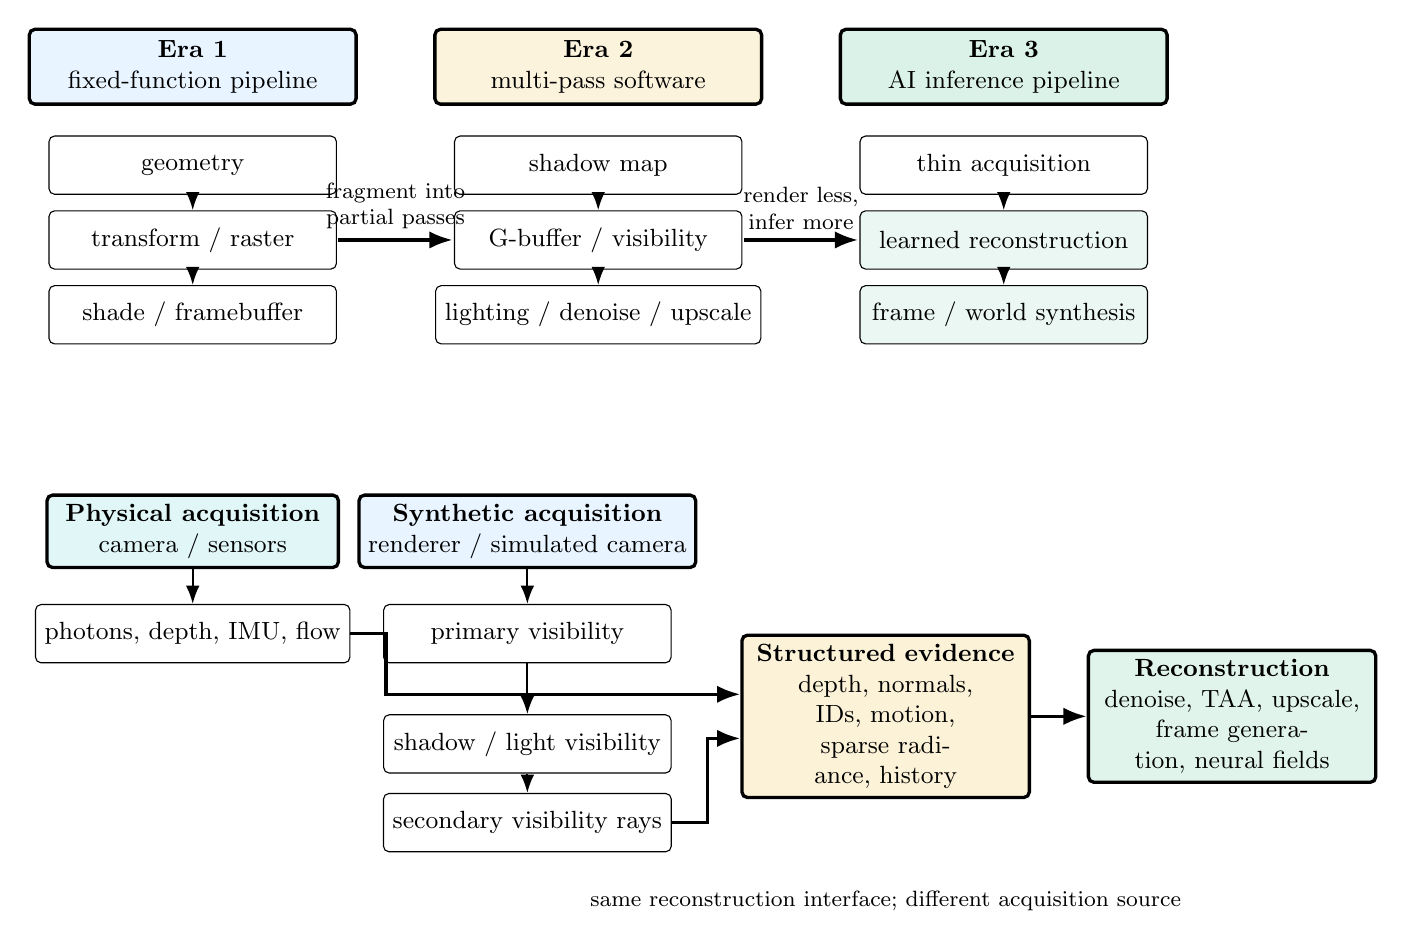
\begin{tikzpicture}[
    font=\small,
    >=Latex,
    era/.style={draw, rounded corners=2pt, very thick, align=center,
        minimum width=4.15cm, minimum height=0.95cm, fill=plotblue!10},
    stage/.style={draw, rounded corners=2pt, align=center,
        minimum width=3.65cm, minimum height=0.74cm, fill=white},
    source/.style={draw, rounded corners=2pt, very thick, align=center,
        minimum width=3.7cm, minimum height=0.9cm, fill=plotcyan!12},
    evidence/.style={draw, rounded corners=2pt, very thick, align=center,
        text width=3.35cm, minimum width=3.65cm, minimum height=1.38cm,
        fill=plotyellow!18},
    recon/.style={draw, rounded corners=2pt, very thick, align=center,
        text width=3.35cm, minimum width=3.65cm, minimum height=1.38cm,
        fill=plotgreen!12},
    arrow/.style={-Latex, thick}
]
% top row: historical rendering eras
\node[era] (era1) at (0,3.15) {\textbf{Era 1}\\fixed-function pipeline};
\node[stage] (era1a) at (0,1.9) {geometry};
\node[stage] (era1b) at (0,0.95) {transform / raster};
\node[stage] (era1c) at (0,0.0) {shade / framebuffer};
\draw[arrow] (era1a) -- (era1b);
\draw[arrow] (era1b) -- (era1c);

\node[era, fill=plotyellow!16] (era2) at (5.15,3.15) {\textbf{Era 2}\\multi-pass software};
\node[stage] (era2a) at (5.15,1.9) {shadow map};
\node[stage] (era2b) at (5.15,0.95) {G-buffer / visibility};
\node[stage] (era2c) at (5.15,0.0) {lighting / denoise / upscale};
\draw[arrow] (era2a) -- (era2b);
\draw[arrow] (era2b) -- (era2c);

\node[era, fill=plotgreen!14] (era3) at (10.3,3.15) {\textbf{Era 3}\\AI inference pipeline};
\node[stage] (era3a) at (10.3,1.9) {thin acquisition};
\node[stage, fill=plotgreen!8] (era3b) at (10.3,0.95) {learned reconstruction};
\node[stage, fill=plotgreen!8] (era3c) at (10.3,0.0) {frame / world synthesis};
\draw[arrow] (era3a) -- (era3b);
\draw[arrow] (era3b) -- (era3c);

\draw[-Latex, very thick] (1.85,0.95) -- node[above, align=center, font=\footnotesize]
    {fragment into\\partial passes} (3.3,0.95);
\draw[-Latex, very thick] (7.0,0.95) -- node[above, align=center, font=\footnotesize]
    {render less,\\infer more} (8.45,0.95);

% bottom row: acquisition equivalence
\node[source] (real) at (0,-2.75) {\textbf{Physical acquisition}\\camera / sensors};
\node[stage] (photons) at (0,-4.05) {photons, depth, IMU, flow};
\draw[arrow] (real) -- (photons);

\node[source, fill=plotblue!10] (synthetic) at (4.25,-2.75) {\textbf{Synthetic acquisition}\\renderer / simulated camera};
\node[stage] (primary) at (4.25,-4.05) {primary visibility};
\node[stage] (shadow) at (4.25,-5.45) {shadow / light visibility};
\node[stage] (secondary) at (4.25,-6.45) {secondary visibility rays};
\draw[arrow] (synthetic) -- (primary);
\draw[arrow] (primary) -- (shadow);
\draw[arrow] (shadow) -- (secondary);

\node[evidence] (evidence) at (8.8,-5.1) {\textbf{Structured evidence}\\depth, normals, IDs, motion,\\sparse radiance, history};
\node[recon] (recon) at (13.2,-5.1) {\textbf{Reconstruction}\\denoise, TAA, upscale,\\frame generation, neural fields};
\draw[-Latex, very thick] (photons.east) -- ++(0.45,0) |- ([yshift=0.28cm]evidence.west);
\draw[-Latex, very thick] (secondary.east) -- ++(0.45,0) |- ([yshift=-0.28cm]evidence.west);
\draw[-Latex, very thick] (evidence) -- (recon);
\node[font=\footnotesize, align=center] at (8.8,-7.45)
    {same reconstruction interface; different acquisition source};
\end{tikzpicture}%
}
\caption{The graphics model that vkGSplat relies on. The upper row shows
the historical shift from a single fixed-function pipeline, to a graph
of partial software passes, to an AI inference pipeline. The lower row
shows the acquisition--reconstruction split: real-world images and
synthetic images differ mainly in the source of acquisition. A real
camera captures physical evidence; a renderer captures structured
evidence from a simulated world through primary visibility, shadow or
light visibility, and secondary visibility. Both then feed
reconstruction.}
\label{fig:graphics-evolution}
\end{figure*}

\subsection{From one pipeline to partial pipelines}

Classical rendering was organized around a relatively direct flow:
geometry entered the pipeline, fixed-function units transformed and
rasterized it, shaders ran at programmable stages, and pixels were
written to a framebuffer~\cite{akenine2018}. Even after vertex and
pixel shaders became programmable, the larger execution model remained
inherited from fixed-function graphics: the shader was programmable,
but the pipeline was not.

Deferred shading changed the abstraction. It separated visibility from
shading by first projecting scene information into screen-space buffers
--- depth, normals, material parameters, motion vectors, and primitive
identity --- and only then shading or filtering those buffers as later
passes~\cite{akenine2018}. Once geometry has been regularized into
screen-space arrays, the problem becomes software-defined: arrays can
be consumed by compute shaders, denoisers, temporal filters, neural
upscalers, and frame-generation models. Modern rendering is therefore
not one pipeline traversal. It is a graph of partial pipelines:
shadow-map passes that need only depth, G-buffer passes that need only
attributes, ray-tracing passes that need sparse secondary visibility,
denoisers that need noisy radiance plus guides, and upscalers that need
a low-resolution frame plus history.

This matters because partial pipelines are much easier to reinterpret
as compute kernels. A shadow pass is a depth-acquisition kernel. A
primary-visibility pass is a camera-acquisition kernel. A
secondary-visibility pass is a sparse sampling kernel. A denoiser or TAA
pass is a reconstruction kernel. Vulkan remains the application-level
description of the work, but the implementation no longer has to be a
hardware raster pipeline.

\subsection{Real and synthetic images share the same reconstruction
contract}

In physical vision, acquisition is sensor capture: photons from the
real world become a noisy, finite-resolution image, often accompanied
by depth, IMU, optical flow, or multi-camera context. In synthetic
vision, acquisition is the early part of the renderer. The renderer is
also a camera, but it observes a simulated world: primary visibility
determines what the virtual camera sees; shadow-map or other
light-visibility passes determine which emitters can contribute;
secondary-visibility rays sample reflection, refraction, indirect
illumination, and occlusion; depth, normals, motion vectors, material
IDs, primitive IDs, and sparse radiance record the evidence.

The source-specific difference is therefore not that one pipeline
produces ``images'' and the other produces ``graphics.'' Both are
acquisition pipelines followed by reconstruction. The only difference is
where the acquisition comes from: a physical camera observing the real
world, or a renderer observing a simulated world. This reframing is
central to vkGSplat. If synthetic acquisition can be implemented as
software visibility and sampling kernels, then the reconstruction path
--- temporal reprojection, history rejection, denoising, super-resolution,
and eventually learned reconstruction --- can live entirely on the same
compute substrate used for training and inference.

\subsection{RT cores, tensor cores, and the new split}

Once the acquisition--reconstruction split is visible, RT cores and
tensor cores no longer look like unrelated add-ons. RT cores accelerate
bounded acquisition: traversal, intersection, and sparse visibility
sampling. Tensor cores accelerate value-scalable reconstruction:
denoising, upscaling, frame generation, neural radiance caching, and
learned scene synthesis. In the language of the modernized Amdahl
framework~\cite{lu2026amdahl}, acquisition is mostly bounded once the
chosen resolution, sample count, and visibility problem are fixed;
reconstruction is value-scalable because additional model capacity and
inference compute keep improving perceptual quality, consistent with AI
scaling behavior~\cite{kaplan2020,lu2026}.

For real-time games, fixed-function acquisition remains valuable because
the frame budget is tight. For SDG, the balance changes. The consumer is
usually a downstream model, not a human staring at a 16-ms deadline, and
the workload is priced in images per dollar or joule. vkGSplat therefore
pushes the split to its logical endpoint: keep the Vulkan description,
but implement both acquisition and reconstruction as tile-friendly
compute.

\subsection{The DLSS precedent: tensor compute is already where the
rendering value lives}
\label{sec:dlss}

The strongest evidence that graphics workloads can move off
graphics-specific silicon is that they already have, partially, inside
NVIDIA's own products. DLSS-class pipelines reduce the renderer's job
from producing the final display image to producing a sparse seed:
sub-native resolution color, depth, motion, and temporally jittered
samples. Neural reconstruction then performs super-resolution,
anti-aliasing, denoising, and, in DLSS~3, frame
generation~\cite{nvidia-dlss,liu2020nsrr,edelsten2019dlss,nvidia-dlss3}.
Ray-traced global illumination follows the same pattern:
single-sample-per-pixel or low-sample path tracing produces sparse
radiance, then spatiotemporal filters and denoisers reconstruct the
image~\cite{schied2017svgf,chaitanya2017interactive,nvidia-nrd,bitterli2020restir}.

vkGSplat does not need to clone DLSS. DLSS is the precedent that proves
the rendering value has already moved toward compute-side
reconstruction. The vkGSplat question is narrower and more actionable:
if the seed is already sparse, noisy, and reconstructed anyway, can a
software renderer produce that seed on AI compute cheaply enough for
SDG? Published software rasterization~\cite{laine2011software}, GPU ray
traversal~\cite{aila2009understanding}, neural supersampling
~\cite{xiao2020}, and compute-native 3DGS~\cite{kerbl20233dgs} make the
answer plausible. vkGSplat is the engineering experiment that turns that
plausibility into a Vulkan-compatible stack.

% =====================================================================
\section{Modernized Amdahl view of the split}
\label{sec:amdahl-main}
% =====================================================================

The companion Amdahl paper reframes the old serial-versus-parallel
question as a hardware-allocation question: with a constrained silicon
or cluster budget, how much should be committed to narrowly specialized
logic, and how much should remain programmable while the workload itself
keeps changing?  The detailed model is in
Appendix~\ref{app:amdahl}; the architectural takeaway is what matters
here.  A fixed-function block is attractive only while it delivers a
large relative efficiency advantage on a stable, value-bounded share of
the workload.  As more of the delivered value moves into stages that
keep improving with model capacity, inference compute, temporal history,
and software updates, the efficiency bar for narrow specialization rises.

This is exactly the structure of modern rendering.  Visibility, shadow
tests, depth, motion vectors, and sparse radiance are bounded acquisition
signals once the camera, resolution, and sample budget are chosen.  The
stage that still scales in value is reconstruction: denoising,
anti-aliasing, super-resolution, frame synthesis, neural radiance
caching, and eventually 3DGS or world-model reconstruction.
Figure~\ref{fig:amdahl-reconstruction-example} shows the same principle in a
small rendering example: a noisy low-sample acquisition can become a
useful image once a reconstruction stage consumes it.

\begin{figure*}[t]
\centering
\begin{minipage}[t]{0.48\textwidth}
\centering
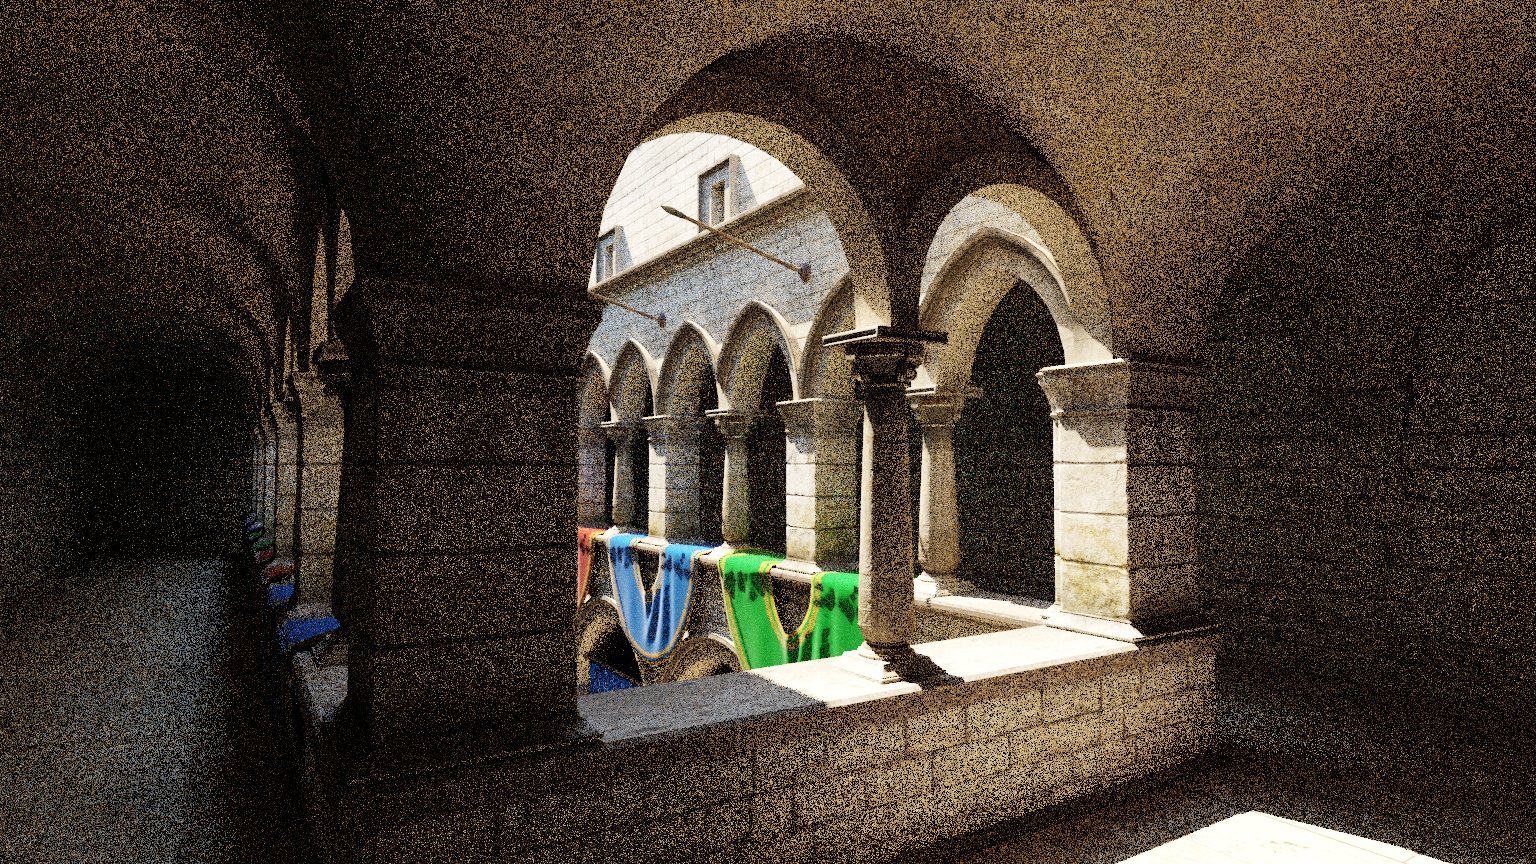
\includegraphics[width=\linewidth]{output/oidn_sponza_noisy.png}

\small \textbf{Low-sample acquisition}
\end{minipage}
\hfill
\begin{minipage}[t]{0.48\textwidth}
\centering
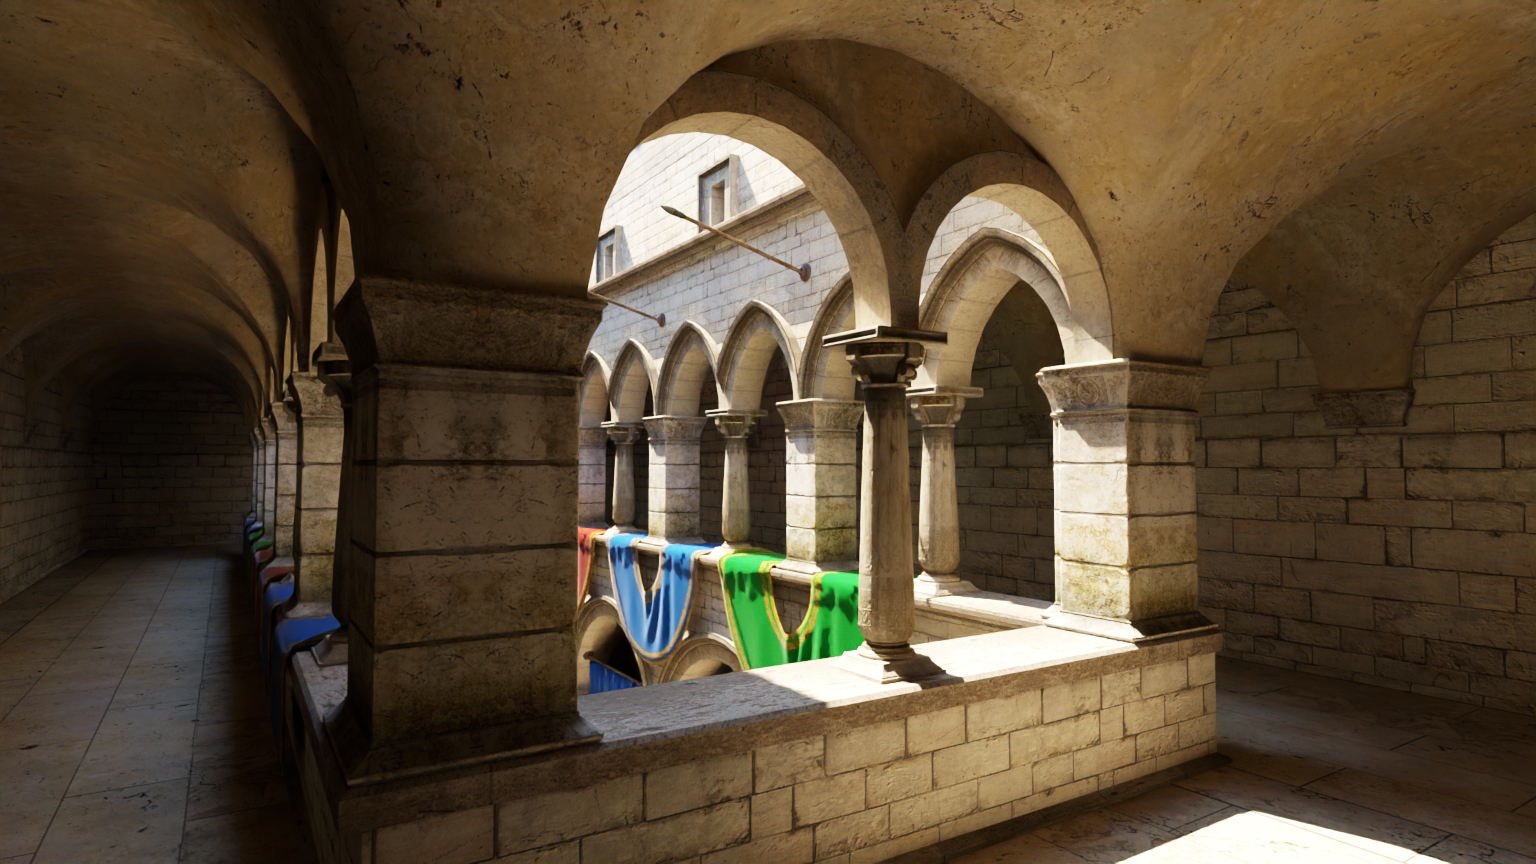
\includegraphics[width=\linewidth]{output/oidn_sponza_denoised.png}

\small \textbf{Reconstructed image}
\end{minipage}
\caption{Rendering as acquisition plus reconstruction.  A low-sample
Monte Carlo image is a sparse, noisy acquisition signal; a denoising or
neural reconstruction stage recovers the image that downstream consumers
actually use.  The example is the Crytek Sponza scene from the Intel
Open Image Denoise gallery~\cite{intel-oidn}.}
\label{fig:amdahl-reconstruction-example}
\end{figure*}

For real-time games, specialized acquisition hardware can remain the
right trade because the 16-ms display budget makes fixed-function
latency valuable.  For SDG, the value function changes.  The consumer is
a training pipeline, not a human display loop, and the economic objective
is images per dollar or joule.  Under the modernized Amdahl view,
vkGSplat deliberately puts the bounded acquisition stages into software
kernels and reserves the programmable substrate for the part of the
pipeline that will keep changing: reconstruction, denoising, temporal
reuse, and learned scene representations.

% =====================================================================
\section{Why SDG is the right workload}\label{sec:workload}
% =====================================================================

\subsection{Throughput-bound, latency-tolerant}

A real-time renderer must finish a frame in $\sim$16~ms or it fails.
A SDG pipeline must produce a target number of labeled images per dollar
or per joule; per-image latency is bounded only by the human iteration
loop and downstream training pipeline. If a software renderer takes
50~ms per image but uses one-tenth the silicon cost of an RTX-class
solution, it wins on $\$\slash\textrm{image}$ even though it loses on
frame time.

Table~\ref{tab:budgets} summarizes the gap between real-time and SDG
per-image budgets. Real-time renderers operate in single-digit-to-tens
of milliseconds, with the constraint that exceeding the budget is
visible to a human user as a dropped frame. SDG pipelines are sized by
the dataset they need to deliver: a typical robotics training run
consumes between $10^5$ and $10^7$ labeled images, the renderer is
allowed minutes per image if necessary, and the binding constraint is
total wall-clock time, dollars, or joules to produce the dataset
rather than per-image latency.

\begin{table}[t]
\centering
\caption{Per-image budgets, real-time vs.\ SDG. Real-time numbers are
the minimum frame budgets needed to avoid visible drops; SDG numbers
are the upper bounds at which a typical training run remains
practical. The relevant figure of merit shifts from \emph{latency} to
\emph{aggregate throughput per dollar / per joule}.}
\label{tab:budgets}
\footnotesize
\setlength{\tabcolsep}{2.5pt}
\renewcommand{\arraystretch}{1.12}
\begin{tabular}{@{}>{\raggedright\arraybackslash}p{0.29\columnwidth}
                >{\raggedright\arraybackslash}p{0.34\columnwidth}
                >{\raggedright\arraybackslash}p{0.27\columnwidth}@{}}
\toprule
& \textbf{Real-time} & \textbf{SDG} \\
\midrule
Per-image budget         & $\leq 16.7$ ms (60\,Hz) & $10^2$--$10^4$ ms \\
                         & $\leq 11.1$ ms (90\,Hz VR)  & \\
Tolerable variance       & low (jitter visible)        & high \\
Resolution               & 1080p--4K display-bound     & 256$^2$--1024$^2$ \\
Images per run           & $\sim$1 (continuous)        & $10^5$--$10^7$ \\
Dominant constraint      & per-frame latency           & throughput, \$/img \\
Hardware preference      & raster + RT cores           & available FLOPS \\
\bottomrule
\end{tabular}
\end{table}

A renderer that produces a $1024{\times}1024$ image in 50~ms is
unusable for real-time, but on a single H100 it would deliver roughly
$1.7{\times}10^6$ images per day. At the same throughput, a 16-GPU pod
produces a 27~M-image dataset per day, which exceeds the size of every
publicly released robotics training dataset to date.

\subsection{Quality requirements}

SDG renderers do not need to convince a human that the image is real;
they need to teach a model that the image is informative. Modern
research~\cite{tobin2017domain,nvidia2024cosmos} suggests that
\emph{diversity}, \emph{labeling fidelity}, and \emph{controlled
randomization} matter more than the marginal photorealism that justifies
RT-core hardware. A 3DGS rendering of a real scene captured with a
phone, augmented with diverse synthetic objects, can be more useful for
training than a mathematically prettier path-traced render of an
unrealistic asset library.

\subsection{Hardware availability and cost}

Table~\ref{tab:hardware} compares the compute economics of the
graphics-class silicon SDG normally targets against the AI-accelerator
silicon teams already own. Two effects compound. First, the
graphics-class lineup (L40, RTX 6000 Ada) ships in much smaller
volumes than the data-center training accelerators: NVIDIA's H100
shipments alone exceeded an estimated three to four million units in
2024, while the L40\slash L40S\slash RTX 6000 Ada production volume is
smaller by roughly an order of magnitude. Second, on a per-unit basis
H100 and B200 deliver $4$--$10{\times}$ more raw FLOPS per dollar of
spot-market rental than graphics-class
parts~\cite{nvidia-hopper-h100,nvidia-blackwell-b200}.

\begin{table}[t]
\centering
\caption{Illustrative per-device specifications and rough order-of-magnitude
spot-market prices~\cite{nvidia-hopper-h100,nvidia-blackwell-b200,nvidia-l40,google-tpu-v5}.
TFLOPS columns report dense BF16\slash FP16 throughput (the regime SDG
kernels run in), not sparse or FP8. Spot prices are illustrative and
fluctuate; we report them only to anchor the cross-class ratios.}
\label{tab:hardware}
\small
\begin{tabular}{@{}lcccc@{}}
\toprule
& \textbf{TFLOPS} & \textbf{HBM/Mem} & \textbf{TDP} & \textbf{Spot \$/hr} \\
& \textit{(BF16)} & (GB) & (W) & \textit{(rough)} \\
\midrule
\textit{AI-accelerator class} & & & & \\
NVIDIA H100 SXM   &  $\sim$990  & 80   & 700  & 2--4  \\
NVIDIA B200       & $\sim$2{,}500 & 192 & 1000 & 4--8  \\
Google TPU v5e    &  $\sim$200  & 16   & 170  & 1--2  \\
AWS Trainium2     &  $\sim$1{,}300 & 96 & ---  & 1--3  \\
\midrule
\textit{Graphics class}       & & & & \\
NVIDIA L40\,/\,L40S         &  $\sim$360  & 48   & 300  & 1--2 \\
NVIDIA RTX 6000 Ada         &  $\sim$364  & 48   & 300  & 1--2 \\
\bottomrule
\end{tabular}
\end{table}

The qualitative point survives any uncertainty in the absolute numbers.
A team that wants to do SDG today is either provisioning a separate
fleet of graphics-class GPUs (competing with rendering studios for a
constrained supply), or running on consumer hardware (RTX 4090, 5090)
that is unstable in data-center deployments. AI compute, by contrast,
is the silicon those teams already operate at scale for training. If
the renderer can run there, the marginal cost of the SDG run is the
opportunity cost of pre-existing capacity rather than the capex of a
new fleet.

A back-of-envelope energy budget reinforces the argument. At a 50-ms
target image budget on an 80\% utilized H100 (700~W TDP), the
rendering energy cost per image is roughly $0.3$~J. At
$10^7$ images, that is $\sim 0.8$ kWh of rendering work --- a
rounding error against the multi-megawatt-hour cost of training the
downstream model.

% =====================================================================
\section{System design}\label{sec:design}
% =====================================================================

vkGSplat is structured as three layers (Fig.~\ref{fig:arch}):

\begin{figure}[t]
\centering
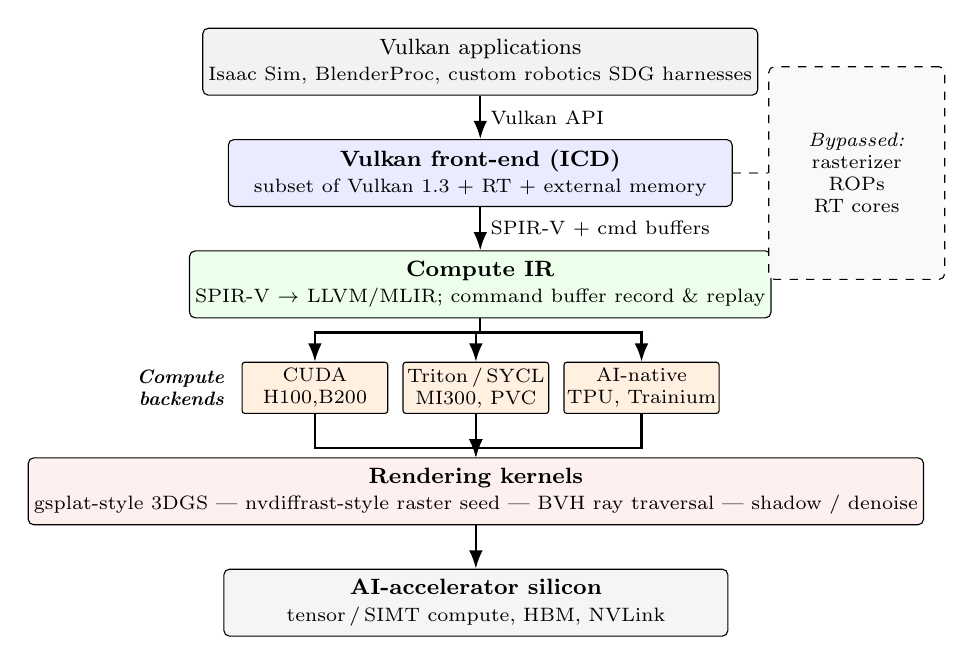
\begin{tikzpicture}[
    font=\footnotesize,
    box/.style    ={draw, rounded corners=2pt, align=center,
                    minimum width=6.4cm, minimum height=0.85cm,
                    inner sep=2pt},
    sub/.style    ={draw, rounded corners=1pt, align=center,
                    minimum width=1.85cm, minimum height=0.65cm,
                    inner sep=1pt, font=\scriptsize},
    arrow/.style  ={-Latex, thick},
    layerlabel/.style={font=\scriptsize\itshape, anchor=west}
]
% --- top: applications ---
\node[box, fill=black!5] (apps) {Vulkan applications\\ \scriptsize Isaac Sim, BlenderProc, custom robotics SDG harnesses};

% --- layer 1: front-end ---
\node[box, fill=blue!8, below=0.55cm of apps] (vk) {%
    \textbf{Vulkan front-end (ICD)}\\
    \scriptsize subset of Vulkan 1.3 + RT + external memory
};

% --- layer 2: IR ---
\node[box, fill=green!8, below=0.55cm of vk] (ir) {%
    \textbf{Compute IR}\\
    \scriptsize SPIR-V $\to$ LLVM/MLIR; command buffer record \& replay
};

% --- layer 3: backends, three side by side ---
\node[sub, fill=orange!12, below=0.55cm of ir, xshift=-2.1cm] (cuda) {CUDA\\\scriptsize H100,B200};
\node[sub, fill=orange!12, right=0.18cm of cuda] (triton) {Triton\,/\,SYCL\\\scriptsize MI300, PVC};
\node[sub, fill=orange!12, right=0.18cm of triton] (ainative) {AI-native\\\scriptsize TPU, Trainium};

% --- bracket label for backends ---
\node[layerlabel, left=0.1cm of cuda, anchor=east, align=right]
    {\textbf{Compute}\\\textbf{backends}};

% --- kernel modules below backends ---
\node[box, fill=red!6, below=0.55cm of triton, minimum width=6.4cm] (kernels)
    {\textbf{Rendering kernels}\\%
     \scriptsize gsplat-style 3DGS~|~nvdiffrast-style raster seed~|~BVH ray traversal~|~shadow / denoise};

% --- silicon ---
\node[box, fill=gray!8, below=0.55cm of kernels] (hw)
    {\textbf{AI-accelerator silicon}\\\scriptsize tensor\,/\,SIMT compute, HBM, NVLink};

% --- arrows down ---
\draw[arrow] (apps) -- node[right]{\scriptsize Vulkan API} (vk);
\draw[arrow] (vk)   -- node[right]{\scriptsize SPIR-V + cmd buffers} (ir);
\draw[arrow] (ir.south) -- ++(0,-0.18) -| (cuda.north);
\draw[arrow] (ir.south) -- ++(0,-0.18) -| (triton.north);
\draw[arrow] (ir.south) -- ++(0,-0.18) -| (ainative.north);
\draw[arrow] (cuda.south)    |- ($(kernels.north)+(0,0.12)$) -- (kernels.north);
\draw[arrow] (triton.south)  -- (kernels.north);
\draw[arrow] (ainative.south)|- ($(kernels.north)+(0,0.12)$) -- (kernels.north);
\draw[arrow] (kernels) -- (hw);

% --- side annotation: existing graphics path crossed out ---
\node[draw, dashed, rounded corners=2pt, align=center, font=\scriptsize,
      right=0.45cm of vk, fill=gray!5, minimum height=2.7cm, text width=2.0cm]
      (notused)
      {\emph{Bypassed:}\\rasterizer\\ROPs\\RT cores};
\draw[dashed,gray] (vk.east) -- (notused.west);

\end{tikzpicture}
\caption{vkGSplat architecture. Applications retain the standard Vulkan
API; the implementation lowers SPIR-V and command buffers to a
backend-agnostic compute IR (LLVM\,/\,MLIR), which is dispatched to
CUDA, Triton\,/\,SYCL, or AI-accelerator-native backends. The
rendering kernels --- 3DGS rasterizer, software tile rasterizer,
BVH ray traversal, denoising --- run as compute on tensor- and
SIMT-rich silicon. The fixed-function graphics path on the GPU is
not used.}
\label{fig:arch}
\end{figure}

\begin{enumerate}
    \item \textbf{Vulkan front-end.} A Vulkan loadable ICD that
    implements a \emph{conformance-targeted subset} of Vulkan~1.3 plus
    selected ray-tracing and external-memory extensions. Mesh shaders
    are treated as the preferred programmable primitive-expansion path
    for Gaussian splats. Tessellation and geometry shaders are not in
    the v1 target: their useful role in this system, expanding compact
    primitives into screen-space work, is subsumed by mesh shaders and
    then by the tile-based software backend. Applications link the
    standard Vulkan loader and need no modification.

    \item \textbf{Intermediate representation (IR).} SPIR-V shaders and
    Vulkan command buffers are lowered into a backend-agnostic compute
    IR. We propose to base this IR on existing infrastructure ---
    LLVM\slash MLIR for shader code, a record-and-replay command-buffer
    IR for pipeline state --- so that the system rides on existing
    compiler ecosystems rather than inventing one.

    \item \textbf{Compute backend.} The IR is lowered to one of several
    backends: CUDA (reference), Triton or SYCL for portability, and
    eventually AI-accelerator-native paths (XLA HLO for TPU, NeuronCore
    for Trainium, etc.). The backend implements the rendering kernels:
    rasterization, ray traversal, shadow mapping, and
    Gaussian-splat blending.
\end{enumerate}

\subsection{Concrete CUDA software stack}

The concrete software stack is now deliberately organized around
CUDA-resident \emph{seed buffers}.  Existing Vulkan programs, beginning
with Wicked Engine workloads, remain the application input.  vkGSplat
captures their command-buffer, descriptor, SPIR-V, camera, and geometry
state, then routes draw and ray-dispatch work into a software CUDA
renderer rather than a fixed-function graphics queue.  The output of
that software renderer is not merely a display image: it is a compact
G-buffer-like seed containing color, depth, primitive identity,
barycentrics or local coordinates, motion-reconstruction inputs, and
optional sample statistics.  Those buffers remain on the CUDA device and
become the direct input to downstream CUDA kernels for screen-space
motion, history reprojection, denoising, temporal antialiasing, and
eventually Gaussian reconstruction.

Three existing CUDA renderers define the source-level reference points.
For triangle visibility, vkGSplat follows the
\textsc{nvdiffrast}/CudaRaster split~\cite{laine2020nvdiffrast}: triangle
setup, bin rasterization, coarse rasterization, and fine rasterization
are separate kernels that produce per-pixel visibility facts such as
depth, triangle identity, and barycentric coordinates.  For canonical
Gaussian visibility, vkGSplat follows the GraphDECO CUDA rasterizer
released with 3DGS~\cite{kerbl20233dgs}: frustum culling and
preprocessing, duplicate Gaussians into tile/depth-keyed work items,
identify tile ranges, and launch tile-local \texttt{renderCUDA}
compositing.  For a broader maintained library reference, vkGSplat also
tracks \textsc{gsplat}~\cite{ye2024gsplat}: fused EWA projection, packed
and unpacked tile intersections, tile-offset construction, flattened
Gaussian IDs, and tile-local front-to-back alpha compositing.  The
important design point is that these paths expose the same kind of
contract --- tile-indexed device buffers --- so the reconstruction stage
does not care whether the seed came from triangle rasterization,
ray-traced visibility, or Gaussian splatting.

This turns the CUDA backend into a producer--consumer pipeline:
\[
\begin{gathered}
\text{Vulkan/Wicked stream}\\
\downarrow\\
\text{CUDA software seed renderer}\\
\downarrow\\
\text{CUDA reconstruction kernels}\\
\downarrow\\
\text{optional CUDA 3DGS renderer}
\end{gathered}
\]
Debug viewers may copy or interop-present the final image, but the
production SDG path should avoid host readback between these stages.
The same buffer ABI is also what CPU and Metal backends must emulate for
correctness testing.

\subsection{Vulkan front-end}

We target a deliberate \emph{subset}: graphics pipelines, compute
pipelines, command buffers, descriptor sets, mesh shaders, indirect
dispatch/draw for GPU-driven splat counts, swapchain (optional, for
debug viewer), timeline semaphores, and external memory. We initially
omit tessellation shaders, geometry shaders, sparse binding, and
presentation-engine optimization. SDG does not need them, and for
Gaussian splatting the tessellation/geometry stages are a worse fit
than mesh shaders followed by tile-local software shading.

\subsection{Lowering rasterization}

We lower the classical raster pipeline to a tile-based software
rasterizer in the spirit of Laine and
Karras~\cite{laine2011software}, with each output tile assigned to a
threadblock\slash workgroup that performs binning, depth test, and
fragment shading.  The immediate implementation reference is
\textsc{nvdiffrast}'s CudaRaster path~\cite{laine2020nvdiffrast}, whose
CUDA stages are explicitly separated into triangle setup, bin raster,
coarse raster, and fine raster kernels.  vkGSplat adopts that staging
but changes the product: instead of a differentiable PyTorch image
operator, the rasterizer emits CUDA-resident seed buffers for SDG
reconstruction. The same organization is used for the 3DGS fast path:
Gaussians are projected once, compacted into screen-space tile lists,
and then blended by tile-local workers. This is the crucial portability
choice. A tile maps naturally to a CUDA cooperative thread array, a SYCL
workgroup, or a TPU/Trainium-style block of dense compute; it also keeps
memory traffic local enough that the backend can be retargeted without
recreating a fixed-function raster pipeline in disguise.

\subsection{Lowering ray tracing and shadow mapping}

Ray-tracing pipelines (\texttt{VK\_KHR\_ray\_tracing\_pipeline}) lower to
software BVH traversal kernels following the
Aila--Laine~\cite{aila2009understanding} pattern, optionally calling
into Embree-like tree construction routines on the host. Shadow maps
become depth-only raster passes followed by a comparison kernel; for
high-quality shadows we expect ray-traced shadows to be cheaper than
classical shadow-map filtering at SDG quality targets.

The seed path is intentionally low-resolution and low-sample. Each
frame exports color, depth, primitive identity, and camera state into
the temporal reconstruction contract. Adjacent frames then provide the
screen-space motion map needed for history lookup; depth and primitive
identity reject disocclusions and visibility changes; a small
SVGF-style filter removes Monte Carlo noise before any optional learned
reconstruction stage is considered.

\subsection{Paused optional 3DGS fast path}\label{sec:v1}

The project previously exposed a non-standard Vulkan extension
(\texttt{VK\_VKGSPLAT\_gaussian\_splatting}) that lets applications submit
Gaussian primitives directly. Internally, this dispatches to a
3DGS rasterizer akin to the GraphDECO CUDA rasterizer released with
3DGS~\cite{kerbl20233dgs}, but extended for offline SDG (deterministic
ordering, deeper sample budgets per pixel, optional denoising).  The
CUDA kernel organization is cross-checked against
\textsc{gsplat}~\cite{ye2024gsplat}: fused EWA projection, tile
intersection, tile-offset construction, flattened Gaussian IDs, and
tile-local pixel compositing. The Vulkan-facing primitive expansion uses mesh shaders:
one workgroup processes a batch of Gaussians, computes view-dependent
color and projected covariance once per splat, and emits the small
screen-space proxy needed by the fragment/tile stage. The production
software backend then keeps the same logical structure but executes it
as explicit tile-binned compute: preprocess, cull, assign splats to
tiles, sort or approximately order within each tile, and blend pixels.

This is why vkGSplat drops tessellation and geometry shaders from the
initial design. Tessellation expands surfaces; geometry shaders expand
or amplify primitives late in the traditional graphics pipeline. For
Gaussian splats, both jobs are better represented by mesh shaders at the
API boundary and by tile-local software work in the backend. A system
that ships this path on day one is immediately useful for captured real
environments and for Lyra-style generated Gaussian scenes. For the
current milestone sequence, however, this path is paused behind a build
flag so the default implementation can focus on Vulkan ray-tracing seed
frames and CUDA lowering.

% =====================================================================
\section{Backends}\label{sec:backends}
% =====================================================================

\textbf{CUDA.} The reference implementation, targeting NVIDIA H100 and
B200. CUDA is mature, has a rich kernel ecosystem (cuBLAS, CUB, Thrust,
OptiX-as-library), and provides external-memory and external-semaphore
interop with Vulkan~\cite{nvidia2020vkcuda}.

\textbf{Triton\slash SYCL.} A second backend in Triton or SYCL would
demonstrate portability and allow deployment on AMD MI300, Intel Ponte
Vecchio, and any future accelerator with an LLVM-class compiler.

\textbf{Metal.} Apple Silicon provides a useful local portability
target. A native Metal backend is not the deployment target, but it
tests whether the reconstruction contracts are genuinely compute
portable rather than CUDA-shaped by accident. We use it first for
temporal reconstruction and denoising on the M-series GPU, then compare
results against the CPU reference before porting the same contracts to
CUDA.

\textbf{AI-accelerator-native.} TPU (XLA HLO), Trainium (NeuronCore SDK),
Cerebras, and Groq each have native compilation paths. Lowering rendering
kernels to these stacks is non-trivial but, for \emph{compute-dominant}
kernels (3DGS rasterization, BVH traversal), feasible. The rendering
problem becomes structurally close to a sparse-attention problem, which
these chips already optimize for.

% =====================================================================
\section{Evaluation plan}
% =====================================================================

We will evaluate vkGSplat along three axes.

\textbf{Throughput.} Images per second at $512^2$ and $1024^2$
resolution on three scene families:
(i)~the standard novel-view-synthesis benchmarks --- Mip-NeRF~360,
Tanks~\& Temples, Deep Blending --- to permit comparison with
published 3DGS numbers~\cite{kerbl20233dgs};
(ii)~SDG-typical procedural scenes from ProcTHOR~\cite{deitke2022procthor}
and a representative subset of Isaac~Lab industrial-manipulation
environments, rendered with controlled domain randomization;
and (iii)~hybrid scenes consisting of a 3DGS-captured real environment
populated with synthetic foreground objects, which is the natural SDG
flow vkGSplat is built for.

\textbf{Cost \& energy.} Dollars-per-image and joules-per-image on a
range of accelerators (H100, B200, A100, L40, MI300, TPU~v5e). The L40
serves as a graphics-hardware baseline; the rest are pure compute.

\textbf{Downstream task accuracy.} Train a small object-detection or
manipulation policy on data generated by vkGSplat vs.\ data generated by
Isaac~Sim or BlenderProc, controlling for total training compute. The
hypothesis is that vkGSplat data is at least competitive on per-dollar
performance.

Concretely, Table~\ref{tab:eval} fixes the matrix we will report.
Each cell is a (scene family, hardware, backend, renderer)
configuration; we report throughput, $\$\slash\textrm{image}$, and
$\textrm{J}\slash\textrm{image}$ as the primary metrics, with PSNR /
SSIM / LPIPS against held-out reference renders for image quality.
Downstream task accuracy is reported on a single curated robotics
benchmark (object-detection mAP on a held-out test set, plus a small
manipulation-policy success rate) rather than chasing a long tail of
benchmarks; the goal is to falsify the hypothesis ``models trained on
vkGSplat data are competitive per dollar with models trained on
Isaac~Sim or BlenderProc data,'' not to exhaustively characterize
sim-to-real transfer.

\begin{table}[t]
\centering
\caption{Evaluation matrix. Each axis is independently varied; the
full Cartesian product is not run --- we ablate one axis at a time
against a reference configuration of \{H100, CUDA, 3DGS,
hybrid 3DGS+synthetic\}.}
\label{tab:eval}
\small
\begin{tabular}{@{}ll@{}}
\toprule
\textbf{Axis} & \textbf{Levels} \\
\midrule
Hardware  & H100, B200, A100, L40S, MI300, TPU v5e \\
Backend   & CUDA (ref), Triton, SYCL, XLA HLO (TPU) \\
Renderer  & 3DGS, software raster, software RT \\
Scene     & Mip-NeRF 360, T\&T, Deep Blending,\\
          & ProcTHOR, Isaac Lab, hybrid 3DGS+CAD \\
Resolution & $512^2$, $1024^2$ \\
\midrule
Metrics   & throughput (img/s), \$/img, J/img, \\
          & PSNR / SSIM / LPIPS, \\
          & downstream mAP, manipulation success \\
\bottomrule
\end{tabular}
\end{table}

% =====================================================================
\section{Discussion}
% =====================================================================

\textbf{When does this lose?} If the workload is dominated by
fixed-function operations (heavy alpha-tested foliage, complex
post-processing chains, high-fidelity displacement), software renderers
on compute will pay a large constant factor. Real-time interactive use
will stay on RTX hardware for the foreseeable future.

\textbf{Why not a new API?} A new graphics API for AI compute has been
proposed informally many times. The reason to keep Vulkan is ecosystem:
existing engines (Unreal's Vulkan RHI, Unity, Godot, Filament), tooling
(RenderDoc, NSight, ImGui), and middleware all speak Vulkan. Reusing
that surface means a vkGSplat backend benefits the ecosystem
asymmetrically.

\textbf{Strategic implications.} If a viable Vulkan-on-AI-compute path
exists, the SDG market is no longer constrained by the supply of
graphics silicon. This is structurally similar to what NVIDIA Omniverse
does for digital twins, but with the asset-distribution and
hardware-binding stories inverted: vkGSplat is open at the API, neutral
at the hardware, and assumes a software-defined data center as its
deployment target. It is also consistent with the direction the
graphics-hardware industry has been moving for half a decade
(Section~\ref{sec:dlss}): each successive generation of DLSS-class
neural reconstruction has shifted more of the rendering pipeline onto
tensor cores. vkGSplat is the architectural endpoint of that
trajectory --- a renderer in which \emph{all} of the work, seed and
reconstruction alike, runs on tensor-rich compute, and graphics
hardware is no longer in the loop.

\textbf{Limitations.} v1 will not be Vulkan-conformant. It will be
correct on a defined subset, on defined drivers, for defined SDG
workloads. Conformance is a long-term goal but not a pre-condition for
usefulness.

% =====================================================================
\section{Related work, expanded}
% =====================================================================

\textbf{Software rasterization.} Beyond the canonical Laine \&
Karras~\cite{laine2011software} result, FreePipe~\cite{liu2010freepipe}
demonstrated programmable parallel rasterization with multi-fragment
effects on GPUs, and Patney \& Owens~\cite{patney2010real} explored
adaptive subdivision on compute. \textsc{nvdiffrast}~\cite{laine2020nvdiffrast}
modernizes the CudaRaster lineage as a set of CUDA-accelerated
graphics primitives --- rasterization, interpolation, texturing, and
antialiasing --- and is the closest existing source-level reference for
vkGSplat's triangle seed renderer. These results predate the modern
tensor-core era but already establish that software-on-compute
rasterization is competitive on workloads where rasterization is not
the bottleneck --- the regime SDG sits in.

\textbf{Differentiable rendering.}
OpenDR~\cite{loper2014opendr} demonstrated that classical rasterizers
could be made approximately differentiable; Li et
al.~\cite{li2018edge} extended this to physically-based path tracing
with edge sampling. The same underlying compute substrate that powers
vkGSplat could host a differentiable variant in future work, allowing
SDG runs to feed gradients back into asset placement or material
parameters.

\textbf{Neural rendering surveys.} Tewari et al.~\cite{tewari2022advances}
surveys the broader space of neural rendering and clarifies that
3DGS sits within a continuum of explicit and implicit
representations. The defining property we exploit ---
compute-native rendering with no fixed-function dependencies --- is
shared with NeRF~\cite{mildenhall2020nerf} and Instant
NGP~\cite{mueller2022instant}, but 3DGS achieves rasterization speeds
that NeRF-class methods do not, which is why we choose it as the v1
renderer.

\textbf{3DGS extensions.} Mip-Splatting~\cite{yu2024mip}
addresses anti-aliasing across scale; 2DGS~\cite{huang20242dgs}
substitutes 2D primitives for tighter geometric fidelity; and
Spec-Gaussian~\cite{yang2024specgaussian} adds anisotropic specular
appearance. The original GraphDECO CUDA rasterizer released with
3DGS~\cite{kerbl20233dgs} is the canonical source reference for the
forward tile-compositing path, while \textsc{gsplat}~\cite{ye2024gsplat}
packages the CUDA projection, tiling, rasterization, batching, and
backward-pass machinery needed for large-scale Gaussian splatting.
vkGSplat targets the original 3DGS forward path first;
incorporating these variants is straightforward because all of them
remain compute-only.

\textbf{API translation precedents.} ANGLE~\cite{angle} translates
OpenGL ES to Direct3D, Metal, or Vulkan, and is the basis for
Chromium's WebGL implementation. VKD3D-Proton~\cite{vkd3dproton}
translates Direct3D~12 to Vulkan and is the engine that allows recent
Windows games to run on Linux under Proton. Both establish that a
shipped, correctness-targeted graphics-API translation layer is
feasible at production scale. vkGSplat's translation goes one step
further by changing not only the API but also the execution
substrate.

\textbf{CUDA--Vulkan interop.} NVIDIA's reference interop
samples~\cite{nvidia2020vkcuda} demonstrate the external-memory and
external-semaphore patterns vkGSplat reuses where the renderer needs
to share images with a Vulkan presentation engine for debug viewers,
even though the production SDG path is headless.

% =====================================================================
\section{Conclusion}
% =====================================================================

We have argued that synthetic data generation for robotics is the wrong
workload to be running on graphics-optimized silicon, and that Vulkan is
the right API to keep. \textbf{vkGSplat} is our proposed bridge: a
software Vulkan implementation whose backend is a compute-only renderer
on AI accelerators, beginning with a 3D Gaussian Splatting fast path
and growing toward a full software graphics stack. The position we
defend is that graphics APIs and graphics hardware should be decoupled,
and that the SDG market is the place where this decoupling pays off
first.

\appendices
\section{Modernized Amdahl allocation details}
\label{app:amdahl}

This appendix integrates the mathematical core of the modernized Amdahl
argument~\cite{lu2026amdahl}.  Classical Amdahl analysis writes
normalized time as
\begin{equation}
  T_A(N) = (1-P) + \frac{P}{N},
  \label{eq:appendix-amdahl}
\end{equation}
where $P$ is the parallelizable fraction and $N$ is processor
count~\cite{amdahl1967}.  Gustafson's law changes the normalization by
allowing workload scale to grow with the machine~\cite{gustafson1988}.
Both forms are useful, but both are phrased around homogeneous
replication.  vkGSplat needs a different question: how should a fixed
resource budget be allocated between specialized graphics logic and
programmable compute when the workload itself is moving?

Let $x \in [0,1)$ be the resource fraction allocated to specialized
logic, let $R>1$ be the relative efficiency advantage of that specialized
logic on the bounded part of the workload, and let $S \in [0,1]$ be the
value-scalable fraction: the share for which additional effective
compute continues to improve quality, capability, or utility over the
design interval.  The first-order allocation objective is
\begin{equation}
  T(x) =
  \frac{1-S}{1+(R-1)x} + \frac{S}{1-x}.
  \label{eq:appendix-allocation}
\end{equation}
The first term is the bounded share helped by specialization; the second
is the scalable share left on programmable compute.  Differentiating,
\begin{equation}
  T'(x)
  =
  -\frac{(1-S)(R-1)}{\left(1+(R-1)x\right)^2}
  + \frac{S}{(1-x)^2}.
  \label{eq:appendix-derivative}
\end{equation}
The objective is strictly convex on $[0,1)$, so the sign of $T'(0)$
determines whether the optimum is interior or collapses to the boundary:
\begin{equation}
  T'(0) < 0
  \quad\Longleftrightarrow\quad
  S < 1 - \frac{1}{R}.
  \label{eq:appendix-threshold}
\end{equation}
Thus, for a fixed specialized efficiency ratio $R$, specialization
collapses when
\begin{equation}
  S_c = 1 - \frac{1}{R}.
  \label{eq:appendix-sc}
\end{equation}
Equivalently, for a fixed scalable fraction $S$, the minimum efficiency
ratio needed to justify specialization is
\begin{equation}
  R_c = \frac{1}{1-S}.
  \label{eq:appendix-rc}
\end{equation}
In the interior regime, solving $T'(x)=0$ yields
\begin{equation}
  x^*
  =
  \frac{\sqrt{\dfrac{(1-S)(R-1)}{S}} - 1}
       {\sqrt{\dfrac{(1-S)(R-1)}{S}} + (R-1)}.
  \label{eq:appendix-optimum}
\end{equation}

\begin{figure}[t]
\centering
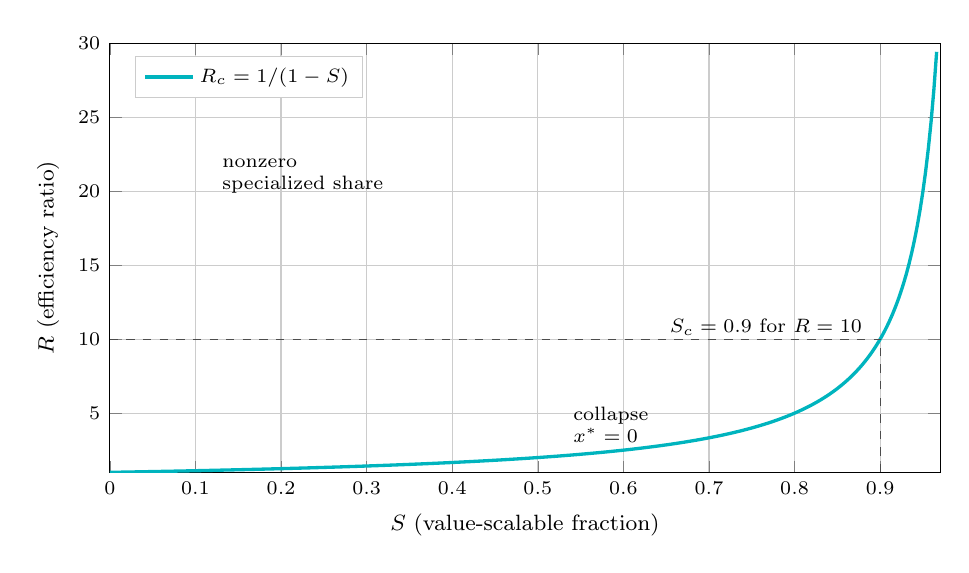
\begin{tikzpicture}
\begin{axis}[
  width=\linewidth,
  height=0.58\linewidth,
  xmin=0, xmax=0.97,
  ymin=1, ymax=30,
  domain=0:0.966,
  samples=300,
  xlabel={$S$ (value-scalable fraction)},
  ylabel={$R$ (efficiency ratio)},
  grid=both,
  grid style={draw=black!10},
  major grid style={draw=black!20},
  ticklabel style={font=\scriptsize},
  label style={font=\footnotesize},
  legend style={font=\scriptsize, cells={anchor=west}, draw=black!20},
  legend pos=north west,
]
\addplot[color=plotcyan, very thick] {1/(1-x)};
\addlegendentry{$R_c = 1/(1-S)$}
\draw[dashed, black!70] (axis cs:0.9,1) -- (axis cs:0.9,10);
\draw[dashed, black!70] (axis cs:0,10) -- (axis cs:0.9,10);
\node[anchor=west, font=\scriptsize, align=left] at (axis cs:0.12,21)
  {nonzero\\specialized share};
\node[anchor=west, font=\scriptsize, align=left] at (axis cs:0.53,4.2)
  {collapse\\$x^*=0$};
\node[anchor=east, font=\scriptsize] at (axis cs:0.89,10.8)
  {$S_c=0.9$ for $R=10$};
\end{axis}
\end{tikzpicture}
\caption{Modernized Amdahl threshold.  As the value-scalable fraction
$S$ rises, the relative efficiency ratio required for a nonzero
specialized allocation rises as $R_c=1/(1-S)$.  This is the mathematical
reason vkGSplat treats fixed-function visibility as bounded acquisition
and keeps reconstruction on programmable compute.}
\label{fig:appendix-amdahl-threshold}
\end{figure}

The interpretation for vkGSplat is direct.  Software visibility, shadow,
and low-sample ray kernels may lose constant factors against dedicated
graphics hardware, but those stages are bounded once they have produced
the seed buffers.  Reconstruction is the value-scalable side: temporal
reuse, denoising, super-resolution, neural fields, and model-driven scene
synthesis can keep absorbing additional effective compute.  As $S$ rises,
the threshold in Fig.~\ref{fig:appendix-amdahl-threshold} says that a
fixed-function graphics block must clear an increasingly high efficiency
bar to justify owning a large fraction of the system.

A bandwidth-limited extension strengthens the same conclusion.  In a
Roofline-style view~\cite{williams2009}, a specialized block may fail to
realize its peak efficiency if memory supply is limiting.  Replacing $R$
with an effective ratio
\begin{equation}
  R_{\mathrm{eff}}(x) =
  \frac{R_{\max}}{1 + \gamma R_{\max}x}
  \label{eq:appendix-reff}
\end{equation}
deforms the interior optimum toward smaller $x$, while the first-order
threshold at the origin remains governed by $S_c=1-1/R_{\max}$.  Memory
pressure therefore reinforces the preference for a broad programmable
substrate in the SDG regime.

\section*{Acknowledgments}
The author thanks the maintainers of the open-source projects this
proposal builds on --- the original 3D Gaussian Splatting team, the
Mesa Lavapipe and SwiftShader communities, the Mitsuba\,/\,Dr.Jit
authors, and the Embree and OptiX teams --- whose work makes the
position defended here a credible engineering target rather than a
speculation. The framing of the DLSS argument owes a debt to the body
of NVIDIA technical writing on real-time neural reconstruction; the
errors in interpreting it are the author's alone.

\bibliographystyle{IEEEtran}
\bibliography{references}

\end{document}
